\documentclass[./dokumentation.tex]{subfiles}

\begin{document}
\chapter{Beziehung/Konflikt von Design, Marketing und Benutzerfreundlichkeit}
Während sich Designer und das Marketing sich häufig darauf konzentrieren, mit leuchtenden Farben und großen Bildern Aufmerksamkeit zu erregen, möchte man im Bereich Usability vor allem Erregungen konzentrieren und negative Emotionen reduzieren, indem sie die Erledigung von Aufgaben erleichtern und sicherstellen. Hier kann es entsprechend zu Konflikten im Produktentwicklungsprozess kommen. 


\section{Emotionaler Einfluss von Farben im Webdesign}
Farben werden in vielen Bereichen eingesetzt, hauptsächlich aus ästhetischen Gründen. Es hat sich gezeigt, dass verschiedene Farben unterschiedliche Wirkungen auf die Psyche haben. Farben treten nicht nur in unserem täglichen Leben auf, Menschen träumen auch in Farbe (\cite{rechtschaffen1992}). Bei normaler Farbsicht, also einer nicht vorhandenen Farbblindheit, können Menschen eine reichhaltige Farbpalette von bis zu 2,3 Millionen unterscheidbaren Farben wahrnehmen (\cite{linhares2008}). Diese Farben lassen sich auf eine beinahe unbegrenzte Art und Weise miteinander kombinieren. \\
Farbentscheidungen begleiten unser tägliches Leben ebenso, sei es die Farbe für eine neue Hose, ein neues Mobiltelefon oder an öffentlichen Plätzen und Gebäuden. \\
Ein Interesse an der Verbindung zwischen Farben und psychologie besteht seit Johann Wolfgang von Goethe, der in seinem Werk “Farbenlehre” bereits einige Spekulationen über die Wirkung von Farben auf die Emotionen des Menschen anstellte. 

Dabei wurden die Farben seitens Goethe in positive und negative Farben eingeteilt. Positiven Farben, wie rot und gelb, wurden nachgesagt, positive Emotionen zu induzieren, wie Wärme und Lebhaftigkeit. Negative Farben, wie blau, violett, wurden mit negativen Emotionen assoziiert, wie Kälte oder Angst.\\

\begin{figure}[H]
    \centering
    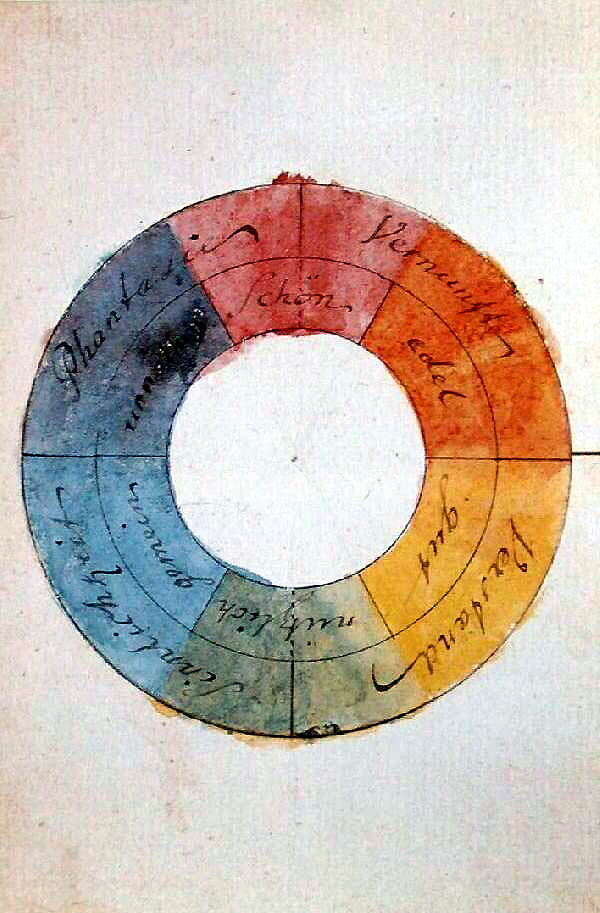
\includegraphics[width=0.5\textwidth]{bilder/goethe.jpg}
    \caption{Goethes erster Farbkreis \cite{goethe1809}}
    \label{fig8:goethe}
\end{figure}\\

Goethes Spekulationen wurden im 20. Jahrhundert vom Psychiater Kurt Goldstein aufgegriffen. Goldstein nahm Goethes Ideen und integrierte sie in die klinische Forschung. Bei seinen Observationen stellte er fest, dass die Farbwahrnehmung physiologische Reaktionen im Körper hervorriefen. Rot und gelb riefen als stimulierende Farben starke Reaktionen hervor, während blau und grün eine beruhigende Wirkung zeigten. Goldsteins Ideen waren vage formuliert und spätere Forscher haben seine Versuche auf die Wellenlänge der Farben übertragen. Farben mit längeren Wellenlängen werden als stimulierend und warm wahrgenommen, während kürzere Wellenlängen als kühl wahrgenommen werden. \\

Heute stellen sich auf Basis dieser Grundlagen weitere Fragen, beispielsweise ob die Farbe einer Bürowand die Produktivität eines Mitarbeiters erhöht, oder ob Farben eine Auswirkung auf den Geschmack von Essen haben (\cite{elliot2004}).\\

Durchgeführte Forschung zur Wirkung von Farben gibt es auch auf die Emotionale Wirkung von Farben beim Spielen von Videospielen. So konnte festgestellt werden, dass die Farbe rot eine starke Erregung und negative emotionale Reaktion hervorruft, während die Farbe gelb eine positive Reaktion verursacht (\cite{joosten}). Es konnte allerdings auch festgestellt werden, dass diese Farbreaktionen insbesondere unerfahrene Spieler betrafen (\cite{joosten}).\\

Ein aktuelles Farbrad mit assoziierten Emotionen lässt sich der Grafik entnehmen. \\

\begin{figure}[H]
    \centering
    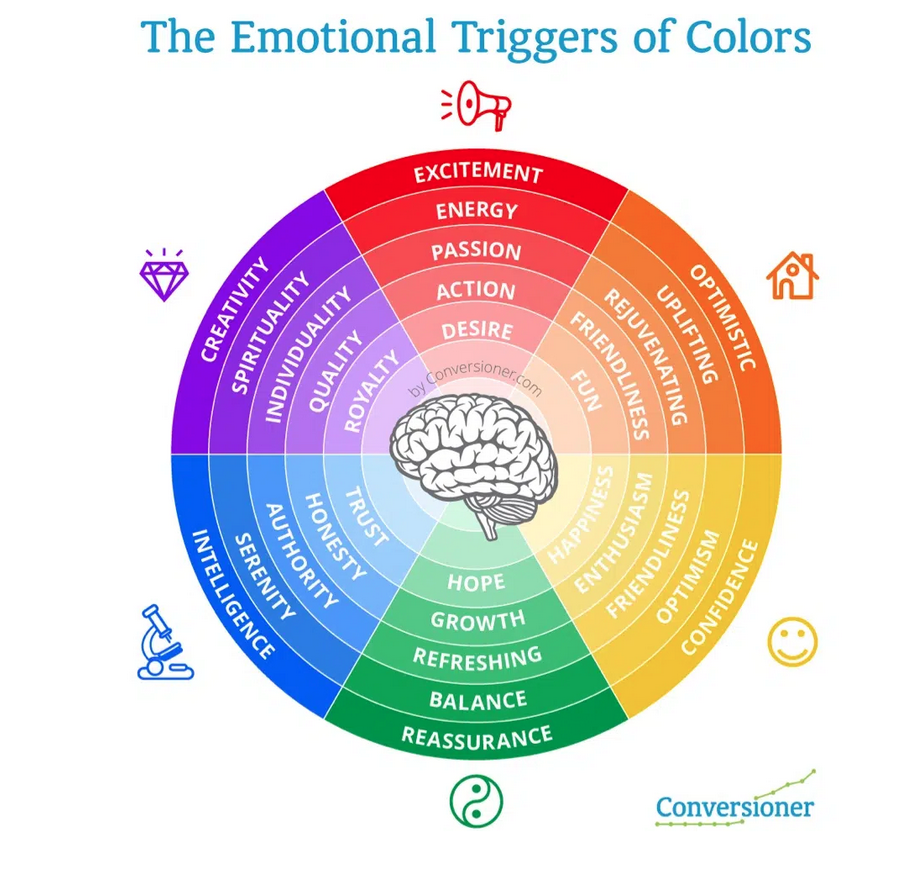
\includegraphics[width=0.8\textwidth]{bilder/farbkreis.png}
    \caption{Ein aktueller Farbkreis \cite{DesignEmo2003}}
    \label{fig9:farbkreis}
\end{figure}\\

\pagebreak

\section{Kulturkreisabhängiges Design und Farbwahrnehmung}
Das Empfinden von Design und damit auch von Farben ist kulturabhängig. Es wurde durch die verschiedenen Lebensweisen in den Kulturen geprägt und ist von gesellschaftlichen und historischen Entwicklungen abhängig. Dabei ist zu beachten, dass dieses Empfinden einem ständigen Wandel unterliegt. Die Symbolwirkung einer Farbe innerhalb eines Kulturkreises kann sich somit nach Jahrhunderten auch plötzlich wandeln. Ein Beispiel für das Wandeln des Farbempfindens ist die Farbe Gelb, die in Korea zunächst traditionell als Farbe für Könige gesehen wurde und sich seit 2000 zunehmend als Trendfarbe, die Hoffnung für das neue Millennium symbolisiert, gewandelt hat. Während Weiß in westlichen Kulturen eher für Reinheit, Glück, Unschuld und Ferne steht, wird diese Farbe in China vor allem mit Tod und Trauer assoziiert. Dies zeigt sich möglicherweise auch in der Gestaltung von YouTube (https://www.youtube.com/) mit viel Weiß und dem chinesischen Pendant YouKu (https://youku.com/), was eher in Schwarz gehalten wurde, wie in Abbildung X zu sehen ist \cite{Kunzer2016}.  \pagebreak



\section{Motivationsquadranten}
Es gibt vier verschiedene Bereiche, die die Konsumenten zu einer Handlung motivieren, die Unternehmen auch im Web einsetzen. Man spricht hier von sogenannten Motivationsquadranten. \\
In Anlehnung an die Cuhelman Emotion Map können wir den Motivationsquadranten in vier verschiedene Emotionen vereinfachen: optimistisch, sicher, pessimistisch und unsicher. \\

\begin{figure}[H]
    \centering
    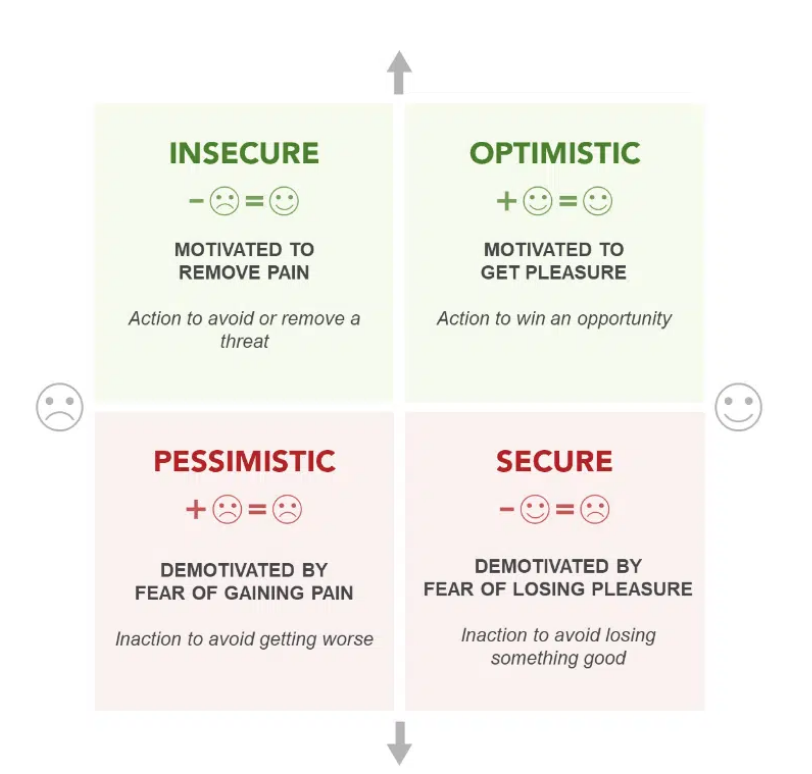
\includegraphics[width=0.8\textwidth]{bilder/motivationsquadranten.png}
    \caption{Motivationsquadranten \cite{designbro}}
    \label{fig9:motivationsquadranten}
\end{figure}\\

\subsection{1. Optimistisch}
Bei diesem Konsumenten besteht das wichtigste Ziel eines Unternehmens darin, einen guten Ruf aufzubauen. Das Unternehmen sollte transparent agieren, ethische Praktiken anwenden und sowohl von Kunden als auch Mitarbeitern geschätzt werden. Konsumenten in diesem Quadranten sind anfällig für Aktionen, sehen kostenlosen Versand und Rückversand als Vorteil und ziehen es in Betracht, affiliate Marketing für das Unternehmen zu betreiben, wenn daraus ein Vorteil entsteht \cite{designbro} \\
 
Zu verwendende Farben: Grün, sowie Hellgrau und Weiß.

\subsection{2. Sicher}
Ihre Kunden sind in ihren Bedürfnissen und Entscheidungen sicher und haben das Gefühl, ihre Erfahrungen mit anderen teilen zu können. Diese Verbraucher schauen sich in der Regel nicht gründlich um und recherchieren nicht gründlich nach Produkten, um sie zu kaufen. Das wichtigste Ziel Ihres Unternehmens besteht darin, diesem Verbraucher dauerhafte, professionelle und lohnende Erlebnisse zu bieten. Kunden sollen sich in Ihrem Unternehmen wohl und verstanden fühlen \cite{designbro}. \\

Zu verwendende Farben: Kühles Blau\\

\subsection{3. Pessimistisch}
Bei diesem Verbraucher besteht das wichtigste Ziel Ihres Unternehmens darin, den Käufer zu belohnen. Durch eine Belohnung entsteht beim Kunden das Gefühl der Wertschätzung. Sie neigen dazu, ihr Geld für schnelllebige Produkte mit hohen Gewinnspannen auszugeben \cite{designbro}. \\

Zu verwendende Farben: Mittel- und Dunkelgrau\\
\subsection{4. Unsicher}
Wenn Sie einen menschlichen Kundendienstmitarbeiter fragen würden, was seiner Meinung nach das häufigste Problem bei Kunden ist, wäre die Antwort wahrscheinlich: Ein unsicherer Kunde, dem die Entscheidungsfindung schwerfällt.\\

Diese Menschen möchten sich wertgeschätzt fühlen und möchten, dass ein Verkäufer ihn langfristig unterstützt, auch wenn es ihm dies durch Aufmerksamkeiten, einen Leitfaden zur digitalen Transformation des Unternehmens oder Treuepunkte einen Mehrwert bietet \cite{designbro}. \\

Zu verwendende Farben: Rot, Orange, Gelb und andere warme Farben; Verwenden Sie es gegen kontrastreiches Schwarz, um optimale Ergebnisse zu erzielen.\\



\end{document}


